\chapter{Requisits del sistema}
\usetikzlibrary{positioning, shadows}
\label{chap:requisits}

Abans d'iniciar el desenvolupament de l'aplicació d'escriptori NUMEN, s'ha dut a terme una anàlisi detallada de requisits, seguint una metodologia rigorosa per garantir l'èxit del projecte. Aquesta fase ha estat clau per identificar les funcionalitats necessàries, establir les característiques tècniques que ha de complir el sistema i definir-ne l'abast, assegurant que la solució final satisfaci les necessitats de l'usuari expert, tant en l'àmbit del càlcul numerològic complex com en la interpretació assistida per Intel·ligència Artificial.

Els requisits s'han classificat en funcionals, no funcionals i de domini, codificant-los per facilitar-ne la traçabilitat i assignant-los una prioritat (alta, mitjana o baixa) en funció de la seva importància per al correcte funcionament del sistema. A més, per facilitar l'anàlisi de dependències i la planificació del desenvolupament, s'han agrupat en blocs lògics.

Tot seguit, es presenta un glossari amb els termes principals utilitzats al llarg d'aquest capítol, per garantir-ne la claredat i coherència terminològica.

\section{Glossari de Termes}

\begin{description}
    \item[App Escriptori] Aplicació dissenyada per a ser executada en ordinadors personals (Windows), que gestiona la interfície d'usuari, la lògica de càlcul local i la comunicació amb serveis externs.
    \item[Backend / Servei IA] Part del sistema (externa a l'app local) que gestiona la comunicació amb els models de llenguatge (LLM) i l'emmagatzematge de dades d'entrenament.
    \item[Usuari] Persona (no professional de la tecnologia) que utilitza el sistema per realitzar estudis numerològics i obtenir interpretacions.
    \item[Administrador] Persona encarregada del manteniment tècnic, la gestió de la base de dades i l'ajust dels *prompts*.
    \item[Figura Espiritual] Representació gràfica dinàmica (triangle o estel) que es construeix visualment en funció dels resultats dels càlculs numerològics de l'usuari.
    \item[Nombres Kàrmics] Nombres específics (13, 14, 16, 19) que indiquen lliçons pendents i que el sistema ha de ressaltar visualment. En el nostre cas concret, hem d'entendre els números kàrmics com números que estan buits (que falten en el nom).
    \item[Inclusió] Esquema numerològic basat en el nom complet, organitzat en una graella on cada posició representa una "Casa" o àrea de la vida.
    \item[Cases] Cadascuna de les 9 àrees de la Inclusió, anomenades també les nou àrees de la vida, que simbolitzen un tret diferent de la personalitat o un àmbit de la vida (ex: Jo, Parella, Treball).
    \item[Habitants] Valor numèric (quantitat de lletres de cert valor) que ocupa una Casa. Representa la intensitat o la manera com es manifesta aquell àmbit en la vida de la persona.
    \item[Prompt] Instrucció textual estructurada que s'envia al model d'Intel·ligència Artificial per guiar la generació de la interpretació.
    \item[RLHF (Reinforcement Learning from Human Feedback)] Procés de millora del model on l'usuari valida les respostes per refinar futurs resultats.
\end{description}

\section{Esquema del Sistema}

El sistema NUMEN compta amb dos actors principals:
\begin{itemize}
    \item \textbf{Usuari:} Persona que utilitza l'aplicació per introduir dades, visualitzar càlculs i obtenir interpretacions.
    \item \textbf{Administrador:} Persona encarregada de la gestió tècnica i supervisió de les dades d'entrenament.
\end{itemize}

A continuació, es mostra un esquema d'alt nivell que reflecteix la interacció entre aquests actors i la plataforma:

\begin{figure}[h]
    \centering
    \begin{tikzpicture}[node distance=2.5cm, auto,
        actor/.style={circle, draw, minimum size=1cm, inner sep=0pt, fill=gray!10},
        block/.style={rectangle, draw, rounded corners, minimum width=2.5cm, minimum height=1.5cm, fill=blue!10, align=center},
        cloudNode/.style={cloud, draw, cloud puffs=10, cloud puff arc=120, aspect=2, minimum width=3cm, fill=green!10, align=center},
        line/.style={draw, -latex', thick}]

        % Nodes
        \node [actor] (user) {Usuari};
        \node [block, right of=user, node distance=4cm] (app) {App Escriptori\\(Càlcul Local)};
        \node [block, right of=app, node distance=4cm] (ai) {Servei IA\\(API)};
        \node [cloudNode, below of=ai, node distance=3cm] (db) {Base de Dades\\(Núvol)};
        \node [actor, left of=db, node distance=4cm] (admin) {Admin};

        % Edges
        % Edges
        \path [line] (user) to[bend left=25] node[above] {Input / Feedback} (app);
        \path [line] (app) to[bend left=15] node[below] {Resultats} (user);
        \path [line] (app) to[bend left=15] node[above] {Prompt} (ai);
        \path [line] (ai) to[bend left=30] node[below] {Interpretació} (app);
        \path [line] (ai) -- node[right] {Dades Entrenament} (db);
        \path [line] (admin) -- node[above] {Gestió} (db);
        \path [line] (admin) -- node[left] {Manteniment} (app);

    \end{tikzpicture}
    \caption{Esquema d'alt nivell del sistema NUMEN.}
    \label{fig:esquema_sistema}
\end{figure}

\section{Requeriments del Sistema}

Els requisits es classifiquen segons el seu tipus: funcionals, no funcionals i de domini. Cada requisit està identificat per un codi únic, indicant també la seva prioritat i l'actor implicat.

\subsection{Requeriments Funcionals}

\begin{table}[H]
    \centering
    \begin{tabular}{|l|l|l|p{8cm}|}
    \hline
    \textbf{ID} & \textbf{Prioritat} & \textbf{Actor} & \textbf{Descripció} \\ \hline
    RF1 & Alta & Usuari & El sistema ha de permetre introduir la data de naixement i els cognoms complets. \\ \hline
    RF2 & Alta & Sistema & El sistema ha de realitzar automàticament els càlculs numerològics (Camí de Vida, Inclusió, etc.). \\ \hline
    RF3 & Alta & Sistema & El sistema ha de mostrar els resultats en el format específic dissenyat (graelles, llistes). \\ \hline
    RF4 & Alta & Sistema & El sistema ha de generar la "Figura Espiritual" dinàmicament segons els resultats. \\ \hline
    RF5 & Alta & Sistema & El sistema ha de detectar i marcar visualment els Nombres Kàrmics (13, 14, 16, 19). \\ \hline
    RF6 & Alta & Usuari & L'usuari ha de poder enviar un prompt a la IA per obtenir una interpretació. \\ \hline
    RF7 & Alta & Sistema & El sistema ha de mostrar la interpretació de la IA en llenguatge natural. \\ \hline
    RF8 & Mitja & Usuari & L'usuari ha de poder valorar la resposta de la IA (feedback) per a l'entrenament. \\ \hline
    RF9 & Alta & Sistema & El sistema ha de guardar la interacció (prompt, resposta, feedback) a la base de dades. \\ \hline
    RF10 & Alta & Usuari & El sistema ha de permetre generar i imprimir un informe final amb els resultats. \\ \hline
    RF11 & Mitja & Admin & L'administrador ha de poder consultar les dades guardades per a re-entrenament. \\ \hline
    RF12 & Baixa & Admin & L'administrador ha de poder configurar els paràmetres de connexió amb la IA. \\ \hline
    \end{tabular}
    \caption{Requisits funcionals del sistema.}
    \label{tab:req_funcionals}
\end{table}

\subsection{Matriu de dependències entre requisits funcionals}

\begin{table}[H]
    \centering
    \resizebox{\textwidth}{!}{%
    \begin{tabular}{|l|c|c|c|c|c|c|c|c|c|c|c|c|}
    \hline
         & \textbf{RF1} & \textbf{RF2} & \textbf{RF3} & \textbf{RF4} & \textbf{RF5} & \textbf{RF6} & \textbf{RF7} & \textbf{RF8} & \textbf{RF9} & \textbf{RF10} & \textbf{RF11} & \textbf{RF12} \\ \hline
    \textbf{RF1} & & X & & & & & & & & & & \\ \hline
    \textbf{RF2} & & & X & X & X & X & & & & X & & \\ \hline
    \textbf{RF3} & & & & & & & & & & X & & \\ \hline
    \textbf{RF4} & & & & & & & & & & X & & \\ \hline
    \textbf{RF5} & & & & & & & & & & X & & \\ \hline
    \textbf{RF6} & & & & & & & X & & X & & & \\ \hline
    \textbf{RF7} & & & & & & & & X & X & X & & \\ \hline
    \textbf{RF8} & & & & & & & & & X & & & \\ \hline
    \textbf{RF9} & & & & & & & & & & & X & \\ \hline
    \textbf{RF10}& & & & & & & & & & & & \\ \hline
    \textbf{RF11}& & & & & & & & & & & & X \\ \hline
    \textbf{RF12}& & & & & & & & & & & & \\ \hline
    \end{tabular}%
    }
    \caption{Matriu de dependències entre requisits funcionals.}
    \label{tab:dependencies_func}
\end{table}

\subsection{Requeriments No Funcionals}

\begin{table}[H]
    \centering
    \begin{tabular}{|l|l|p{5cm}|p{5cm}|}
    \hline
    \textbf{ID} & \textbf{Prioritat} & \textbf{Descripció} & \textbf{Verificació} \\ \hline
    RNF1 & Alta & La interfície ha de ser intuïtiva per a usuaris sense perfil tècnic. & Test d'usabilitat amb l'usuari final (menys de 2 errors en el primer ús). \\ \hline
    RNF2 & Mitja & El temps de resposta de la IA ha de ser inferior a 10 segons. & Mesura de temps de resposta en 20 peticions consecutives. \\ \hline
    RNF3 & Alta & Compatibilitat amb Windows 10 i 11. & Prova d'instal·lació i execució en màquines virtuals i físiques. \\ \hline
    RNF4 & Alta & Integritat de les dades emmagatzemades per a RLHF. & Verificació de consistència a la base de dades després de 50 insercions. \\ \hline
    RNF5 & Mitja & L'aplicació ha de permetre la impressió en format A4 sense desconfiguració. & Prova d'impressió física i en PDF. \\ \hline
    \end{tabular}
    \caption{Requisits no funcionals del sistema.}
    \label{tab:req_nofuncionals}
\end{table}

\subsection{Requeriments del Domini}

\begin{table}[H]
    \centering
    \begin{tabular}{|l|l|p{10cm}|}
    \hline
    \textbf{ID} & \textbf{Prioritat} & \textbf{Descripció} \\ \hline
    RD1 & Alta & Els càlculs han de seguir estrictament la metodologia de Martine Coquatrix (reducció teosòfica, excepcions). \\ \hline
    RD2 & Alta & La interpretació de la IA ha de ser respectuosa, constructiva i empàtica. \\ \hline
    RD3 & Mitja & Privacitat: No s'han de guardar dades personals identificables (PII) a la base de dades d'entrenament, només els càlculs i resultats. \\ \hline
    RD4 & Alta & El sistema ha de reconèixer correctament els Nombres Mestres (11, 22, 33) i no reduir-los en els contextos adequats. \\ \hline
    RD5 & Alta & La Figura Espiritual ha de respectar la geometria sagrada definida en el marc teòric. \\ \hline
    \end{tabular}
    \caption{Requisits del domini.}
    \label{tab:req_domini}
\end{table}

\section{Matriu de dependències entre tots els requisits}

\begin{table}[H]
    \centering
    \resizebox{\textwidth}{!}{%
    \begin{tabular}{|l|c|c|c|c|c|c|c|c|c|c|c|c|c|c|c|c|c|c|c|c|c|c|}
    \hline
         & \textbf{RF1} & \textbf{RF2} & \textbf{RF3} & \textbf{RF4} & \textbf{RF5} & \textbf{RF6} & \textbf{RF7} & \textbf{RF8} & \textbf{RF9} & \textbf{RF10} & \textbf{RF11} & \textbf{RF12} & \textbf{RNF1} & \textbf{RNF2} & \textbf{RNF3} & \textbf{RNF4} & \textbf{RNF5} & \textbf{RD1} & \textbf{RD2} & \textbf{RD3} & \textbf{RD4} & \textbf{RD5} \\ \hline
    \textbf{RF1} & & X & & & & & & & & & & & & & & & & & & & & \\ \hline
    \textbf{RF2} & & & X & X & X & X & & & & X & & & & & & & & X & & & X & \\ \hline
    \textbf{RF3} & & & & & & & & & & X & & & X & & & & & & & & & \\ \hline
    \textbf{RF4} & & & & & & & & & & X & & & & & & & & & & & & X \\ \hline
    \textbf{RF5} & & & & & & & & & & X & & & & & & & & & & & & \\ \hline
    \textbf{RF6} & & & & & & & X & & X & & & & & X & & & & & & & & \\ \hline
    \textbf{RF7} & & & & & & & & X & X & X & & & X & & & & & & X & & & \\ \hline
    \textbf{RF8} & & & & & & & & & X & & & & & & & & & & & & & \\ \hline
    \textbf{RF9} & & & & & & & & & & & X & & & & & X & & & & X & & \\ \hline
    \textbf{RF10}& & & & & & & & & & & & & & & & & X & & & & & \\ \hline
    \end{tabular}%
    }
    \caption{Matriu de dependències global.}
    \label{tab:dependencies_global}
\end{table}

\section{Relació amb la Planificació}

Per garantir que tots els requisits definits siguin coberts durant el desenvolupament, s'ha establert una relació directa entre els Paquets de Treball (PT) definits al Capítol \ref{Chapter4} i els requisits del sistema.

La Figura \ref{fig:mapa_requisits} mostra visualment aquesta distribució, assegurant que cada bloc funcional del projecte té assignats els seus objectius tècnics específics.

\begin{figure}[H]
    \centering
    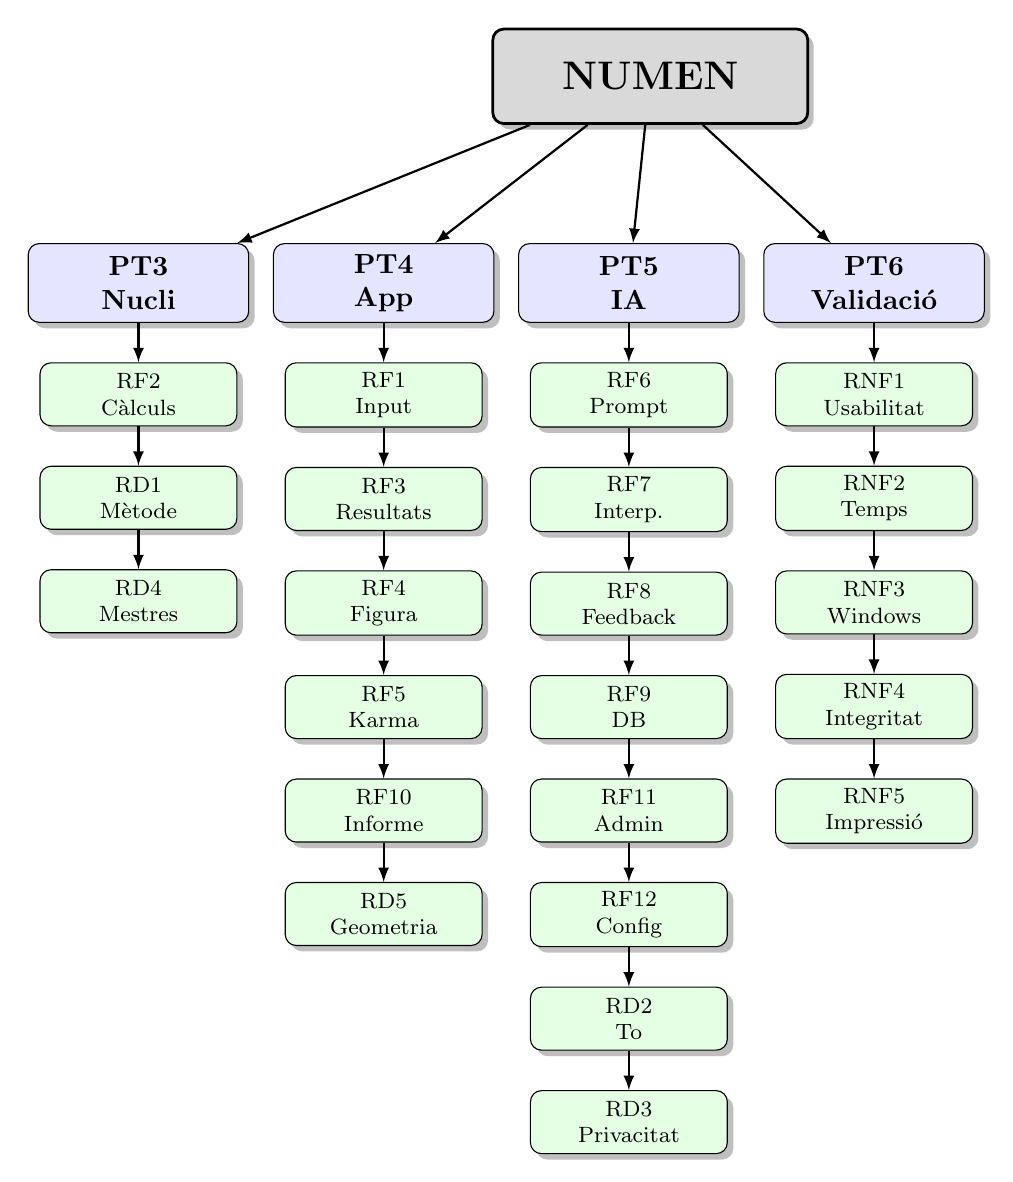
\begin{tikzpicture}[
        node distance=0.5cm and 0.2cm,
        every node/.style={draw, rounded corners, align=center, font=\small, fill=white, drop shadow},
        root/.style={fill=gray!30, font=\Large\bfseries, minimum width=4cm, minimum height=1.2cm, line width=1pt},
        pt/.style={fill=blue!10, font=\bfseries, minimum width=2.8cm, minimum height=1cm},
        req/.style={fill=green!10, font=\footnotesize, minimum width=2.5cm, minimum height=0.8cm},
        link/.style={-latex, thick}
    ]

    % Root
    \node[root] (root) {NUMEN};

    % Level 1: PTs (Horizontal distribution)
    \node[pt, below=1.5cm of root, xshift=-6.5cm] (pt3) {PT3\\Nucli};
    \node[pt, right=0.3cm of pt3] (pt4) {PT4\\App};
    \node[pt, right=0.3cm of pt4] (pt5) {PT5\\IA};
    \node[pt, right=0.3cm of pt5] (pt6) {PT6\\Validació};

    % Edges Root -> PTs
    \draw[link] (root) -- (pt3);
    \draw[link] (root) -- (pt4);
    \draw[link] (root) -- (pt5);
    \draw[link] (root) -- (pt6);

    % Level 2: Requirements (Vertical Stacks)
    
    % PT3 Children (Nucli: Càlculs, Mètode, Mestres)
    \node[req, below=0.5cm of pt3] (rf2) {RF2\\Càlculs};
    \node[req, below=of rf2] (rd1) {RD1\\Mètode};
    \node[req, below=of rd1] (rd4) {RD4\\Mestres};
    \draw[link] (pt3) -- (rf2);
    \draw[link] (rf2) -- (rd1);
    \draw[link] (rd1) -- (rd4);

    % PT4 Children (App: Input, Resultats, Figura, Karma, Informe, Geom)
    \node[req, below=0.5cm of pt4] (rf1) {RF1\\Input};
    \node[req, below=of rf1] (rf3) {RF3\\Resultats};
    \node[req, below=of rf3] (rf4) {RF4\\Figura};
    \node[req, below=of rf4] (rf5) {RF5\\Karma};
    \node[req, below=of rf5] (rf10) {RF10\\Informe};
    \node[req, below=of rf10] (rd5) {RD5\\Geometria};
    \draw[link] (pt4) -- (rf1);
    \draw[link] (rf1) -- (rf3);
    \draw[link] (rf3) -- (rf4);
    \draw[link] (rf4) -- (rf5);
    \draw[link] (rf5) -- (rf10);
    \draw[link] (rf10) -- (rd5);

    % PT5 Children (IA: Prompt, Interp, Feedback, DB, Admin, Tone, Privacy)
    \node[req, below=0.5cm of pt5] (rf6) {RF6\\Prompt};
    \node[req, below=of rf6] (rf7) {RF7\\Interp.};
    \node[req, below=of rf7] (rf8) {RF8\\Feedback};
    \node[req, below=of rf8] (rf9) {RF9\\DB};
    \node[req, below=of rf9] (rf11) {RF11\\Admin};
    \node[req, below=of rf11] (rf12) {RF12\\Config};
    \node[req, below=of rf12] (rd2) {RD2\\To};
    \node[req, below=of rd2] (rd3) {RD3\\Privacitat};
    \draw[link] (pt5) -- (rf6);
    \draw[link] (rf6) -- (rf7);
    \draw[link] (rf7) -- (rf8);
    \draw[link] (rf8) -- (rf9);
    \draw[link] (rf9) -- (rf11);
    \draw[link] (rf11) -- (rf12);
    \draw[link] (rf12) -- (rd2);
    \draw[link] (rd2) -- (rd3);

    % PT6 Children (Validació: Usabilitat, Temps, Windows, Integritat, Impressió)
    \node[req, below=0.5cm of pt6] (rnf1) {RNF1\\Usabilitat};
    \node[req, below=of rnf1] (rnf2) {RNF2\\Temps};
    \node[req, below=of rnf2] (rnf3) {RNF3\\Windows};
    \node[req, below=of rnf3] (rnf4) {RNF4\\Integritat};
    \node[req, below=of rnf4] (rnf5) {RNF5\\Impressió};
    \draw[link] (pt6) -- (rnf1);
    \draw[link] (rnf1) -- (rnf2);
    \draw[link] (rnf2) -- (rnf3);
    \draw[link] (rnf3) -- (rnf4);
    \draw[link] (rnf4) -- (rnf5);

    \end{tikzpicture}
    \caption{Mapa conceptual de relació entre Paquets de Treball i Requisits.}
    \label{fig:mapa_requisits}
\end{figure}
